\documentclass[12pt,a4paper]{scrreprt}
% Языки, которые могут быть использованы.
\usepackage[english,russian]{babel}

% FreeSerif — альтернатива TimesNewRoman
\usepackage{fontspec}
\setmainfont[Ligatures=TeX]{Times New Roman}
\setmonofont[Mapping=,Ligatures=]{Courier New}

% Чтобы сделать буковки ещё красивее.
\usepackage{microtype}

% Картинки, вращение и всё такое. Причём даже в режиме черновика
\usepackage[final]{graphicx}
\usepackage{float}
\usepackage[draft=no]{svg}
\usepackage{pdfpages}

% Чтобы легко менять стиль списков
\usepackage[shortlabels]{enumitem}

\usepackage{unicode-math}
\usepackage{csquotes}
\usepackage{adjustbox}
\usepackage{relsize}

% https://tex.stackexchange.com/questions/14967/source-code-listing-with-frame-around-code
\usepackage{listings}
\lstset{frame=lrbt,xleftmargin=\fboxsep,xrightmargin=-\fboxsep}
\lstset{basicstyle=\ttfamily,breaklines=true}

% https://qna.habr.com/answer?answer_id=1140867
\bibliographystyle{gost2008}
\usepackage[
	style=gost-numeric, % стиль цитирования и библиографии, см. документацию biblatex-gost
	language=auto,  % использовать язык из babel
	autolang=other, % многоязычная библиография
	parentracker=true,
	backend=biber,
	hyperref=true,
	bibencoding=utf8,
	sorting=ntvy,  % сортировка: имя, заголовок, том, год
]{biblatex}
\addbibresource{bibliography.bib}
\DeclareSourcemap{
    \maps{
        \map{% если @online, то устанавливаем media=eresource.
            \step[typesource=online, fieldset=media, fieldvalue=eresource]
        }
    }
}

% Отсупы как по госту.
\usepackage[
	includeheadfoot,
	left=20mm,
	right=10mm,
	top=0mm,
	headheight=25mm,
	footskip=5\baselineskip, % footskip is the distance between the textbody and the baseline of the footer
	bottom=15mm,
]{geometry}

\savegeometry{original}
\geometry{bottom=10mm}
\savegeometry{nofooter}
\loadgeometry{original}

%% Некоторые переменные, которые появляются более одного раза

% Название курсовой. Не забывать проценты в конце строк.
\newcommand{\docTitle}{%
	Сервис для индексирования и просмотра репозиториев%
}

\newcommand{\docTitleEng}{%
	Repository Indexing and Viewing Service%
}

% Год написания курсовой.
\newcommand{\YEAR}{
	\the\year{}
}

% RU — код страны
% 17701729 — код НИУ ВШЭ
% 05.15 — регистрационный номер (https://docs.cntd.ru/document/566085681)
% 		В данном случае, Прикладное ПО / Информационные системы для решения специфических отраслевых задач
% 01 — номер редакции документа
% 33 — код вида документа (https://www.swrit.ru/doc/espd/19.101-77.pdf#page=4)
% 01 — номер документа данного вида
%  1 — номер части документа
\newcommand{\docId}{RU.17701729.03.10-01 12 01-1}


% Footer and header
\usepackage{fancyhdr}
\pagestyle{fancy}
\fancyhf{}
\chead{
	%\bf % Сделать жирненьким
	\thepage\\
	\docId
}
\fancyhead[RO]{%
    % В правый верхний колотитул пихаю номер приложения
    {\ifnum\value{addendum}>0 ПРИЛОЖЕНИЕ \theaddendum \fi}
}
\cfoot{%
	\adjustbox{valign=b}{ % baseline of footer at bottom, so margins are correct
		\begin{tabular}{| l | l | l | l | l |}
			\hline & & & & \\
			\hline Изм. & Лист & № докум. & Подп. & Дата \\
			\hline \docId &  &  &  &  \\
			\hline Инв. № подл. & Подп. и дата & Взам. инв. № & Инв. № дубл. & Подп. и дата № \\
			\hline
		\end{tabular}
	}
}
\fancypagestyle{nofooter}{%
	\fancyfoot{}%
}

\renewcommand{\headrulewidth}{0pt}
\renewcommand{\footrulewidth}{0pt}

% Повернуть на 90 градусов
\newcommand{\rot}[2]{\rotatebox[origin=c]{90}{\enspace\parbox{#1 - 0.5em}{#2}}}

% Повторить #1 раз текст #2: \Repeat{#1}{#2}
\usepackage{expl3}
\ExplSyntaxOn
\cs_new_eq:NN \Repeat \prg_replicate:nn
\ExplSyntaxOff

% Продвинутые таблицы
\usepackage{tabularx}
\usepackage{multirow}
\usepackage{xltabular}
% И сразу делаем чтобы колонки X центрировались по вертикали
\def\tabularxcolumn#1{m{#1}}
\newcolumntype{Y}{>{\centering\arraybackslash}X}

% Подсчет числа страниц
\usepackage{lastpage}

% Расчет всяких размеров
\usepackage{calc}

% Названия разделов по центру (но titlesec конфликтует с hyperref)
\usepackage{titlesec}
\titleformat{\section}
  {\centering\Large\bfseries}
  {\thesection}
  {.5em}
  {\MakeUppercase}
% И с точкой в конце.
\titlelabel{\thetitle.\quad}

% После названия раздела надо делать отступы у абзацев.
\usepackage{indentfirst}

% https://tex.stackexchange.com/a/347803
\usepackage{varwidth}

\newcommand{\placename}{
	\underline{\hspace{4cm}}
}
\newcommand{\placedate}{
	«\underline{\hspace{1em}}» \underline{\hspace{3cm}} \YEAR г.
}

\newcounter{addendum}
\makeatletter
\newcommand{\addendum}[1]{
    \stepcounter{addendum}

	% Приложения есть в оглавлении
	\phantomsection
	\addcontentsline{toc}{section}{Приложение \arabic{addendum}: #1}

	\section*{#1}
	
	% Сбросить все счетчики
	\setcounter{equation}{0}
    \setcounter{figure}{0}
    \setcounter{table}{0}

	% Треш и угар с макросами, чтобы обойти проблемы между titlsec и hyperref
	% Цель: \NR@gettitle{Приложение 1: …}, но нужно **сначала** раскрыть \arabic{addendum}
	\edef\addendumTitle{\noexpand\NR@gettitle{Приложение \arabic{addendum}: #1}}
	\addendumTitle
}
\makeatother

% Ещё больше подсекций
\newcommand{\subsubsubsection}[1]{\paragraph{#1}\mbox{}\\}
\setcounter{secnumdepth}{4}
\setcounter{tocdepth}{4}

% TODOшечки
\usepackage{ifdraft}
\ifdraft{
	% Если \document[draft], то нам нужно место в полях для todo.
	\geometry{left=40mm, right=5mm, marginparwidth=35mm}
	\reversemarginpar  % причём слева они выглядят симпатичнее
	\savegeometry{original}
}{}
\usepackage[obeyDraft,textsize=footnotesize,textwidth=35mm]{todonotes}

% Добавляем гипертекстовое оглавление в PDF
% hyperref должен быть последним
\usepackage[hidelinks]{hyperref}
\usepackage[nonumberlist,nogroupskip,xindy={glsnumbers=false,codepage=utf8,language=russian}]{glossaries}
\usepackage[automake=immediate]{glossaries-extra}
% \setabbreviationstyle[acronym]{short-footnote}
\setglossarystyle{list}
\renewcommand{\glossarysection}[2][]{}
\renewcommand{\glsnamefont}[1]{\textrm{#1}}
\makeglossaries

\newglossaryentry{IDE}
{
    name=IDE,
    description={(Integrated Development Environment) — интегрированная среда разработки, предоставляющая разработчику большое количество функционала для работы с кодом проектов}
}

\newglossaryentry{LSP}
{
    name=LSP,
    description={(Language Server Protocol) \cite{lsp-book} — разработанный Microsoft протокол взаимодействия редактора кода и специального сервиса, который способен анализировать код проекта и предоставлять редактору продвинутый функционал, сравнимый с классическими IDE}
}

\newglossaryentry{LSIF}
{
    name=LSIF,
    description={(Language Server Index Format) \cite{lsif} — специальный формат, в котором LSP-сервер может вывести информацию о проекте таким образом, что её можно переиспользовать в дальнейшем, не имея при этом запущенного экземпляра сервера и даже кода проекта}
}

\newglossaryentry{symbol}
{
    name={Символ},
    text={символ},
    description={(в контексте исходного кода) — идентифкатор в тексте программе, однажды где-либо определенный. Например, в строке «\texttt{def func():}» символом будет являться «\texttt{func}». Также символами являются имена переменных, классов и многое другое}
}

\newglossaryentry{repo}
{
    name={Репозиторий},
    text={репозиторий},
    description={— файлы какого-либо программного проекта, включающие, среди прочего, весь его исходный код. В данной работе под репозиторием имеется ввиду Git-репозиторий, в котором все файлы также находятся под управлением системы контроля версий Git, которая позволяет эффективно создавать новые версии репозитория и делиться внесенными изменениями с другими разработчиками}
}

\begin{document}
	\selectlanguage{russian}

	\newenvironment{LeftTablePage}{%
	\thispagestyle{empty}%
	% Временно уменьшаем отступы.
	\newgeometry{left=5mm, top=25mm, bottom=10mm}%
	% Содержимое слева.
	\noindent\begin{minipage}[b]{20mm}
		\rotatebox{90}{
			\begin{tabular}{| c | c | c | c | c |}
				\hline
				Инв. № подл. & Подп. и дата & Взам. инв. № & Инв. № дубл. & Подп. и дата \\
				\hline
				\docId & & & & \\
				\hline
			\end{tabular}%
		}
	\end{minipage}%
	% Основное содержимое
	\begin{samepage}%
	\begin{minipage}[b][\textheight]{\textwidth}\centering%
}{
	\end{minipage}%
	\end{samepage}
	
	% Теперь можно вернуть отступы как были
	\restoregeometry

	\clearpage
}

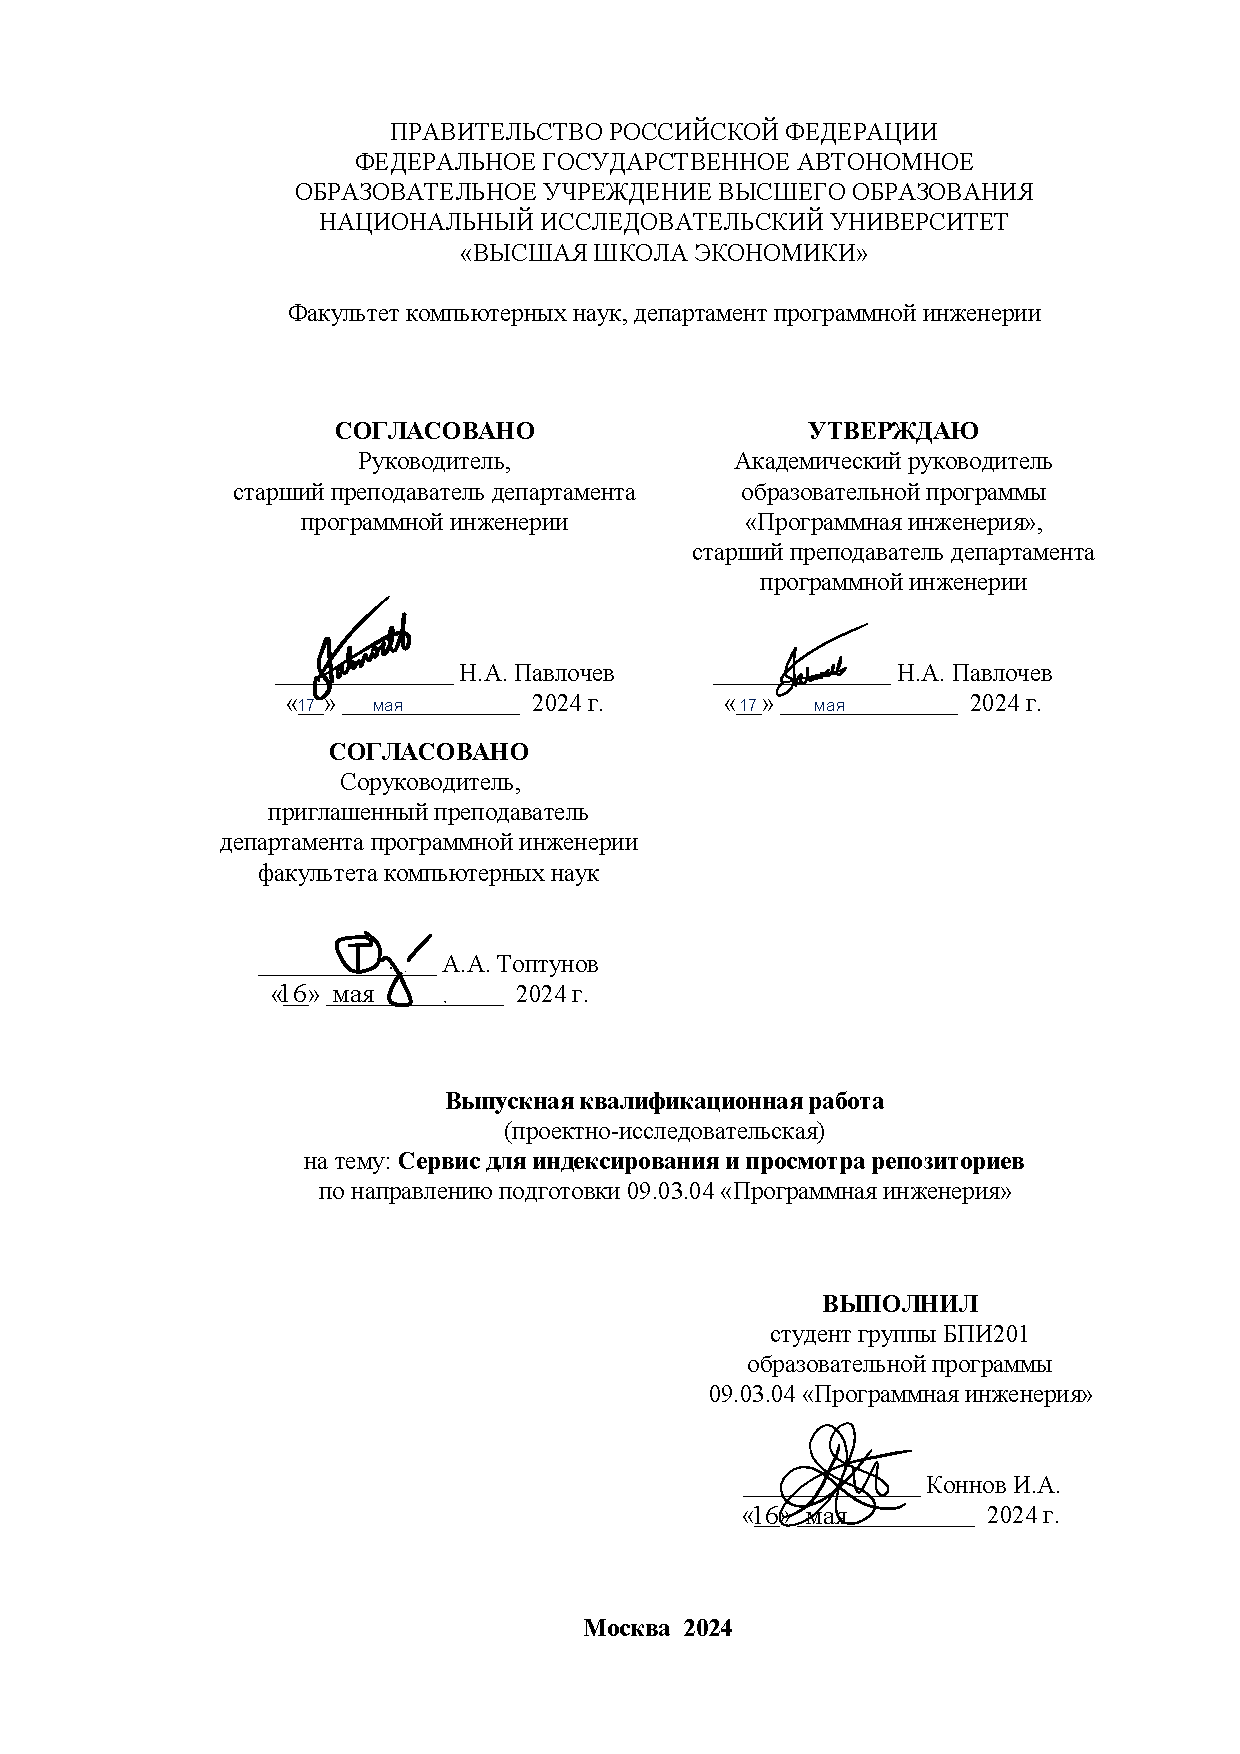
\includepdf[pages=-]{figures/signed.pdf}
% \begin{LeftTablePage}
% 	%% Лист утверждения
    ПРАВИТЕЛЬСТВО РОССИЙСКОЙ ФЕДЕРАЦИИ \\
    ФЕДЕРАЛЬНОЕ ГОСУДАРСТВЕННОЕ АВТОНОМНОЕ \\
    ОБРАЗОВАТЕЛЬНОЕ УЧРЕЖДЕНИЕ ВЫСШЕГО ОБРАЗОВАНИЯ \\
    НАЦИОНАЛЬНЫЙ ИССЛЕДОВАТЕЛЬСКИЙ УНИВЕРСИТЕТ \\
    «ВЫСШАЯ ШКОЛА ЭКОНОМИКИ» \\[1\baselineskip]
    Факультет компьютерных наук, департамент программной инженерии
\vskip 1.5cm
    % Согласовано / утверждаю
    \begin{varwidth}[t]{0.45\textwidth}\centering
    	\textbf{СОГЛАСОВАНО}
    	
    	Руководитель, \\
    	старший преподаватель департамента
        программной инженерии
    \end{varwidth}%
    \hfil%
    \begin{varwidth}[t]{0.45\textwidth}\centering
    	\textbf{УТВЕРЖДАЮ}
    	
    	Академический руководитель
        образовательной программы
        «Программная инженерия», \\
        старший преподаватель департамента
        программной инженерии
    \end{varwidth}

\bigskip

    \begin{varwidth}[t]{0.4\textwidth}\centering
    	\placename Н.А. Павлочев \\
    	\placedate
    \end{varwidth}%
    \hfil%
    \begin{varwidth}[t]{0.4\textwidth}\centering
    	\placename Н.А. Павлочев \\
    	\placedate
    \end{varwidth}

\bigskip

    \begin{minipage}[t]{0.45\textwidth}\centering
    	\textbf{СОГЛАСОВАНО}
    	
    	Соруководитель, \\
    	приглашенный преподаватель
        департамента программной инженерии
        факультета компьютерных наук
    \end{minipage}%
    \hfil\makebox[0.45\textwidth]{}

\bigskip

    \begin{minipage}[t]{0.45\textwidth}\centering
    	\placename А.А. Топтунов \\
    	\placedate
    \end{minipage}%
    \hfil\makebox[0.45\textwidth]{}

\vfill

    \textbf{\uppercase{\docTitle}}

    \bigskip

    Программа и методика испытаний

    \bigskip

    \textbf{
    	\Large
    		ЛИСТ УТВЕРЖДЕНИЯ \\
    	\large
    		{\docId} 01-1-ЛУ \\
    	\normalsize
    		Листов \pageref*{LastPage}
    }

\vfill

    \makebox[0.45\textwidth]{}\hfil%
    \begin{minipage}[t]{0.45\textwidth}\centering
    	\textbf{ВЫПОЛНИЛ}
            
    	студент группы БПИ201 \\
    	образовательной программы \\
    	09.03.04 «Программная инженерия» \\
    \end{minipage}

\bigskip

    \makebox[0.45\textwidth]{}\hfil%
    \begin{minipage}[t]{0.45\textwidth}\centering
    	\placename Коннов И.А. \\
    	\placedate
    \end{minipage}

\vskip 1.5cm

    \textbf{Москва \YEAR}
% \end{LeftTablePage}

% ГОСТ гласит, что лист утверждения не должен быть нумероваться: титульный лист это первый лист
\pagenumbering{arabic}

\begin{LeftTablePage}
	%% Первые две страницы ТЗ:
%% 1. Лист утверждения
%% 2. Титульный лист

\begin{flushleft}
\begin{varwidth}{\linewidth}\centering
	\large
	УТВЕРЖДЕН \\
	{\docId} 01-1-ЛУ
\end{varwidth}
\end{flushleft}

\vskip4cm

{\Large\uppercase{\docTitle}}

\vskip1cm

{\large
	Текст программы

	{\docId} 01-1
}

\vskip1cm

Листов \pageref*{LastPage}

\vfill
\textbf{Москва \YEAR}
\end{LeftTablePage}
	
	
	% На всякий случай, хотя вообще не очень нужно.
	\loadgeometry{original}
	
	\addsec{Реферат}

Данная работа посвящена реализации сервиса для индексирования Git-репозиториев, предоставляющего функционал навигации по исходным кодам репозитория с возможностью найти определение тех или иных символов, или всех их использований. Подобная система позволяет оптимизировать работу разработчиков и помочь им при изучении кода программных проектов.

Сначала приводится сравнение с существующими аналогичными решениями, формулируются проблемы и список требований к реализуемой системе. Затем в тексте предлагаются решения поставленных проблем и приводятся конкретные методы для получения и хранения исходных текстов из Git-репозиториев, для получения семантических данных и для эффективного формирования ответа на запросы с использованием технологии LSIF, а также предлагается способ версионирования данных для хранения различных версий репозитория в одной базе данных. В том числе описывается механизм для быстрого получения семантических данных в ущерб их точности, используя информацию из раннее проиндексированных версий репозитория. Наконец, в этом документе приводятся детали реализации системы: общая архитектура, используемые технологии, описание модели данных и описания отдельных сервисов, а также протоколы их взаимодействия друг с другом.

Работа содержит \pageref*{LastPage} страниц, \total{chaps} главы, \totalfigures{} рисунков, \total{citenum} источников, \total{addendum} приложений.

\textit{Ключевые слова: репозиторий, индексация, Git, language server, контроль версий}

\clearpage

\addsec{Abstract}

This work is devoted to the implementation of a service for indexing Git repositories, which provides functionality for navigating through the source codes of the repository with the ability to find the definition of certain symbols or all their uses.

First, a comparison with existing similar solutions is given, problems are formulated and a list of requirements for the system being implemented. Then the text suggests solutions to the problems posed and provides specific methods for obtaining and storing source texts from Git repositories, for obtaining semantic data and for effectively forming a response to queries using LSIF technology, as well as a method for versioning data to store different versions of the repository in one database. In particular, it describes a mechanism for quickly obtaining semantic data at the expense of their accuracy, using information from earlier indexed versions of the repository. Finally, this document provides details of the system implementation: the overall architecture, the technologies used, a description of the data model and descriptions of individual services, as well as protocols for their interaction with each other.

This work contains \pageref*{LastPage} pages, \total{chaps} chapters, \totalfigures{} figures, \total{citenum} references, \total{addendum} appendicies.

\textit{Keywords: repository, indexing, Git, language server, graph, version control}


\clearpage

    {
        \singlespacing
		\renewcommand*\contentsname{\centering Содержание\vspace{-6pt}}
		\tableofcontents
    	\clearpage
	}

	% Основное содержимое
	\addsec{Основные определения, термины и сокращения}

\printglossary[nonumberlist]

\clearpage
	\addsec{Введение}

При разработке программного обеспечения часто необходимо читать исходный код проектов, причем разработчик может быть первоначально не знаком с изучаемым исходным кодом. Это часто случается при изучении поведения внешних систем или при недостатке документации. При этом для облегчения понимания кода разработчику помогают специальные инструменты, которые способны анализировать код и помогать в изучении проекта.

Такие инструменты должны предоставлять следующий функционал:
\begin{itemize}
    \item Отображение подсказки при наведении курсора на \gls{symbol} в исходном коде: информация о типе переменной, документация.
    \item Переход к определению символа. Это может быть переход к определению функции от места её использования, что часто бывает полезно для изучения процесса обработки данных в программе. Это также может быть переход к определению типа от места его использования, что позволит увидеть содержащиеся в нём поля.
    \item Поиск всех использований символа — обратный функционал к операции перехода к определению символа. Например, позволяет найти все места, где вызывается функция, и исходя из этого лучше понять её входные параметры.
\end{itemize}

Обычно для этого применяются \gls{IDE}, которые требуют скачивания проекта на компьютер разработчика и затем достаточно длительной загрузки всех зависимостей, компиляции и индексации. До завершения этих операций IDE не способна проанализировать и предложить разработчику подсказки. Это значительно замедляет изучение сложных систем, состоящих из многих отдельных сервисов.

Однако существует возможность значительно уменьшить время от необходимости изучать код проекта до получения подсказок, если заранее и централизованно индексировать \gls{repo}, ещё до того как данные индексации понадобятся разработчикам. Можно выполнять компиляцию и индексацию на каждом новом изменении в репозитории, чтобы, при необходимости, актуальные данные всегда были доступны.

Такой подход позволит обеспечить разработчикам быстрый и удобный доступ к функционалу навигации по коду без необходимости выполнения длительной и ресурсоёмкой индексации. Однако создание такой системы требует решения многих задач: хранения данных репозитория и индексов, реализация пользовательского интерфейса, предоставление частичных ответов в условии отсутствия актуальных индексов по тем или иным причинам.

Подобные системы разработаны во многих больших компаниях, занимающихся разработкой программного обеспечения (Google, Facebook\facebook, Yandex), но обычно такие системы доступны только их сотрудников и очень тесно интегрированы с проприетарными системами сборки. Также существует несколько открытых аналогов и коммерческие системы, но те обладают своими недостатками. В этой работе приводятся методы решения задач индексации, а также приводится описание реализованной системы индексирования Git-репозитория.

Выпускная квалификационная работа состоит из введения, трех глав и заключения:

\begin{itemize}
    \item В \hyperref[chap:overview]{\textbf{первой главе}} дается постановка проблемы и анализируются возможные пути её решения.
    \item Во \hyperref[chap:solution]{\textbf{второй главе}} описываются основные идеи и алгоритмы разработанной системы.
    \item В \hyperref[chap:architecture]{\textbf{третьей главе}} рассматривается архитектура системы и описываются детали её реализации.
    \item В \hyperref[chap:final]{\textbf{заключении}} резюмируется функциональный и технический подход к разработке системы.
\end{itemize}

\clearpage

	\chapter{Обзор предметной области и анализ существующих решений}
\label{chap:overview}

\section{Предметная область}

При разработке программного обеспечения часто необходимо читать код смежных проектов, чтобы уточнить детали поведения, прояснить особенности API, или найти существующую реализацию определенной функциональности.
Также часто используется система хранения версий Git \cite{git-paper}, а также какая-либо платформа для организации совместной работы над проектами (например, GitLab, BitBucket).
Эти платформы предоставляют возможность с использованием веб-интерфейса читать код проектов, но не предоставляют возможностей по навигации, сравнимых с возможностями полновесной \gls{IDE}.
Это сильно усложняет процесс погружения в незнакомые проекты, потому что разработчик лишается привычных подсказок (например, вывод типов, документация) и возможностей по навигации (например, go to definition).
Обычно эти возможности доступны только при локальном выкачивании проекта и последующем его индексировании с помощью \gls{IDE}, однако это занимает достаточно много времени.
Особенно ситуация усугубляется при использовании микросервисной архитектуры, когда количество репозиториев становится большим.

Таким образом, у разработчиков существует потребность в решении, которые бы предоставляло им продвинутые возможности навигации и поиска по коду, но без необходимости трудоемкого индексирования.
Индексация кода должна осуществляется автоматически и асинхронно, в то время как разработчики должны иметь возможность использовать ранее построенные индексы с использованием специального приложения.

Особенно остро эта проблема стоит в связи с нынешней проблемой в продлении лицензий на многие коммерческие продукты.

\section{Существующие решения}

Для индексации кода существует множество различных существующих решений, рассмотрим некоторые из них:

\begin{itemize}
    \item SourceBrowser \cite{SourceBrowser} для .NET — позволяет сгенерировать для проекта статический сайт с возможностью перейти к определению любого \glslink{symbol}{символа} и возможностью найти все использования того или иного символа. Однако, поддерживает только языки на базе .NET.
    
    \item Google CodeSearch \cite{rsc-regexp4} — осуществляет быстрый regexp-поиск по кодовой базе, но не осуществляет никакого семантического анализа. На данный момент не поддерживается.
    
    \item The Elixir Cross Referencer \cite{elixir-crossrefrencer} — отлично индексирует код на C/C++, но не поддерживает другие языки.
    
    \item Glean \cite{facebook-Glean} — система, решающая задачу хранения данных индексации и выполнения запросов к ним. Но она не предоставляет удобного веб-интерфейса, а также до сих пор находится в разработке.
    
    \item SourceGraph \cite{miljenovic2010sourcegraph} — эффективно решает все индексации и навигации проблемы, но на данный момент больше не является открытым и бесплатным решением.
\end{itemize}

Все эти решения либо не являются открытыми и бесплатными, либо поддерживают только очень ограниченное количество языков программирования, либо не предоставляют необходимый функционал.

\section{Требования к системе}

Таким образом, можно сформулировать основные требования к системе:

\begin{enumerate}
    \item Система должна иметь открытый исходный код и распространяться под свободной лицензией;
    \item Система должна иметь возможность индексировать код на различных языках программирования. Обязательно должны поддерживаться языки программирования Rust и TypeScript;
    \item Система должна предоставлять функционал поиска определения символа, поиска всех использований символа и отображение справочной информации при наведении курсора на символ;
    \item Система должна иметь веб-интерфейс, в котором пользователь сможет просматривать содержимое репозитория;
    \item Система должна быть простой в развертывании и использовании;
    \item Система должна иметь возможность ограниченно использовать индексы построенные с использованием предыдущей версии репозитория даже при просмотре той версии, которая ещё не была проиндексирована.
\end{enumerate}

\section{Выводы по главе}

С одной стороны, система решает действительно важную и актуальную проблему разработчиков. Она может позволить заметно облегчить их работу и уменьшить время решения некоторых задач. С другой стороны, хотя аналоги и существуют, но на данный момент не было найдено аналогичных решений, распространяемых под свободной лицензией, поэтому разработка системы весьма актуальна. Также были сформулированы основные требования к этой системе.

\clearpage
	\chapter{Алгоритмы и методы решения}
\label{chap:solution}

\section{Получение исходных текстов}

Прежде чем индексировать данные, необходимо научиться их автоматически получать и помещать в хранилище для дальнейшего доступа.

Предполагается, что в качестве системы контроля версий используется Git. Поэтому предлагаемое решение использует особенности его работы, чтобы более эффективно сохранять данные.

Git хранит всё содержимое репозитория с использованием двух видов объектов: \textbf{деревья} (trees) и файлы (blobs). Каждое дерево представляет собой директорию и хранит в себе список своих непосредственных потомков: всех поддеревьев и всех файлов. Каждый объект является неизменяемым и имеет уникальный идентификатор. В случае, если содержимое файла не изменилось, то его идентификатор не меняется и переиспользуется объект из предыдущего состояния репозитория. В случае же, если в файле были некоторые изменения, то создается новый объект файла и содержащее его \textbf{дерево} клонируется таким образом, чтобы указывать на новую версию файла (и старые версии неизменившихся файлов). Аналогично изменения распространяются до самого корня репозитория. Всё это позволяет указывать на любую версию репозитория с помощью единственного идентификатора корневого \textbf{дерева}, и при этом переиспользовать неизменившиеся между версиями объекты.

Чтение данных напрямую из репозитория, однако, довольно затруднено. С одной стороны, Git не позволяет эффективных способов доступа к отдельным объектам без выкачивания всего репозитория (потому что объекты, бывает, группируются и сжимаются вместе). С другой стороны, доступ к серверу часто ограничен авторизацией и большая читающая нагрузка может создать на него неожиданную нагрузку. Для обхода этих ограничений, предлагаемый Сервис хранит копию всех данных из Git-репозитория в собственной базе данных.

Процесс синхронизации изменений выглядит следующим образом:

\begin{enumerate}
    \item При помощи команды \texttt{git pull} на диск выкачивается актуальное состояние репозитория;
    \item Чтением объектов из директории \texttt{.git} определяется текущее корневое дерево и собирается список всех файлов и всех директории в текущем состоянии репозитория. При этом пропускаются все директории и файлы, которые уже были обработаны ранее.
    \item Найденные объекты загружаются в базу данных.
\end{enumerate}

Это позволяет эффективно находить все изменения в репозитории и не дублировать файлы в хранилище Сервиса.

К сожалению, Git не позволяет общего метода узнавать об изменениях, кроме как периодически проверяя их наличие. Сервис предоставляет все механизмы для индексации того или иного репозитория, но его запуск возлагается на пользователя — это может быть настроенный на создание новых коммитов webhook на стороне сервиса вроде Gitlab или Bitbucket, или может быть cron-задача, индексирующая репозиторий время от времени.

\section{Получение семантических данных}

Исходя из сформулированных требований, помимо получения текстового содержимого репозитория, также необходимо получить семантическую информацию о коде: информация о символах в коде и связях между ними.

Учитывая необходимость индексировать различные проекты на различных языках программирования, нужно использовать универсальный и расширяемый метод для индексации. Существует несколько разных подходящих механизмов получения необходимой информации:

\begin{itemize}
    \item Google Kythe \cite{Kythe} — одна из первых попыток предоставить независящий от языка API для получения информации о коде. Несмотря на богатые возможности, проект не пользуется популярностью вне Google, а количество поддерживаемых языков весьма ограничено.
    \item Language Server Index Format (LSIF) \cite{lsif} — формат, построенный вокруг экосистемы Language Server. Имеет детальную документацию и поддерживается большим количеством языков программирования (за счет отдельных анализаторов исходного кода для каждого языка).
    \item SCIP Code Intelligence Protocol (SCIP) \cite{scip} — развитие LSIF для применения внутри Sourcegraph. Более эффективен, чем LSIF, но сложнее в интеграции и использовании.
\end{itemize}

Исходя из простоты использования и наиболее широкой поддержкой сообществом, для реализации был выбран \gls{LSIF}.

Модель \gls{LSIF} представляет собой граф, в котором описываются различные виды узлов и описываются связи между ними. Ключевым для данного проекта является вид узлов, соответствующим подстрокам в исходном коде индексируемого проекта. Так, например, для следующего кода будет, среди прочих, найдено два узла, представляющие собой подстроки «foo» и «self».
\begin{minted}{Python}
def foo(self):
    pass
\end{minted}

Каждая подстрока задается номером строки, началом и длиной, а также может иметь тег. Затем эти для этих подстрок в графе формируются ребра, описывающие результаты вызова метода Language Server (например, \texttt{textDocument/definition}) по отношению к этим подстрокам, а также их принадлежность к тем или иным файлам.

При обработке графа, выполняется две задачи. Во-первых, все подстроки привязываются к ранее загруженному в базу данных файлу из Git-репозитория. Во-вторых, в базу данных копируются все ребра и узлы графа. Причем важно понимать, что результат индексирования одного файла могут меняться при изменении совершенно других. Эта особенность требует также реализовать механизмы версионирования и для всех объектов, описывающие граф. Более подробно модель данных описывается в разделе \fullref{section:data-model}.

\section{Пользовательский интерфейс}

Пользовательский интерфейс реализован с помощью специальной сборки Visual Studio Code, которая работает прямо в браузере пользователя. Встроенное в неё расширение обеспечивает взаимодействие с бекендом: отображение всех файлов, предоставление подсказок, функциональность навигации.

Расширение решает три задачи:
\begin{enumerate}
    \item Предоставляет реализацию виртуальной файловой системы, доступной только на чтение и загружающее файлы и деревья с сервера.
    \item Указывает для VSCode способ взаимодействия с реализацией \gls{LSP}, работающей на бекенде.
    \item Предоставляет команды для выбора текущей версии репозитория.
\end{enumerate}

Бекенд, в свою очередь представляет API для доступа к:

\begin{enumerate}
    \item Списку версий репозитория (со ссылкой на корневую директорию этой версии);
    \item Доступ к объектам файлов и объектам директорий;
    \item API для выполнения LSP-запросов, с указанием используемой версии репозитория.
\end{enumerate}

Все запросы к API осуществляются с помощью HTTP. Более подробно оно описывается в разделе \fullref{section:api}.

\section{Алгоритм формирования ответа на запрос LSP-клиента}
\label{lsp-algorithm}

Среди всех видов вершин графа \gls{LSIF} можно выделить наиболее важные:
\begin{itemize}
    \item \texttt{Range} — вершины, указывающие на некоторую подстроку в файле;
    \item \texttt{[…]Result} — вершины, хранящие результат того или иного запроса;
    \item \texttt{ResultSet} — вершины, агрегирующие результаты для нескольких похожих подстрок. Например, для одной и той же функции «get» во всех местах будет отображаться одна и та же информация при наведении курсора, независимо от конкретного места использования функции.
\end{itemize}

Также рассмотрим некоторые виды рёбер:

\begin{itemize}
    \item \texttt{Next} — соединяет вершину \texttt{Range} и все связанные с ней вершины \texttt{ResultSet}.
    \item \texttt{Item} — для каждой вершины-результата связывает с ней подстроки, которые входят в ответ.
    \item \texttt{Definition}, \texttt{Hover}, \texttt{References} и т.п. — соответствуют методам запросов в протоколе \gls{LSP} и связывают \texttt{ResultSet} с соответствующими результатами запросов.
\end{itemize}

\begin{figure}[H]
    \centering
    \includesvg[inkscapelatex=false, width=\textwidth, height=0.5\textheight]{figures/lsif.svg}
    \caption{Изображение подграфа, содержащего информацию о функции «get».}
    \label{fig:lsif-graph}
\end{figure}

Алгоритм ответа на запрос «найти определение \glslink{symbol}{символа}, расположенного в файле $D$ под $N$-ым символом на строке $L$, используя версию репозитория $V$» будет состоять из следующих операций:

\begin{enumerate}
    \item Найти в базе данных объект файла $D$.
    \item Найти в нём строку $L$.
    \item Найти в базе данных все проиндексированные подстроки, которые содержатся внутри найденной строки $L$ и одновременно в версии $V$.
    \item Среди них выбрать те подстроки, которые включают в себя $N$-ый символ (на рисунке соответствующая подстроке вершина графа выделена цветом).
    \item Для данных подстрок, используя ребра \texttt{Next}, найти все связанные с ними узлы типа \texttt{ResultSet}.
    \item Найти в графе рёбра с типом \texttt{Definition}, связывающие найденные \texttt{ResultSet} и узел, содержащий результат запроса. Ожидается найти только единственный такой.
    \item \label{item-definitions} Найти в графе ребро с типом \texttt{Item}, соединенное с результатом запроса. Другими словами, найти все узлы графа, которые входят в данный результат.
    \item Это ребро будет соединять результат запроса с подстрокой, соответствующей искомому определению.
    \item Для подстроки можно найти файл, в котором та находится, а затем, с использованием всей этой информации, сформировать ответ пользователю.
\end{enumerate}

Аналогичным образом можно находить все использования символа (в п. \ref{item-definitions} алгоритма необходимо выбирать ребра со свойством «References»), а также отвечать на любые другие запросы, необходимые в рамках данного проекта.

\section{Версионирование данных}

Поскольку сервис допускает просмотр различных версий репозитория, остро встает вопрос об эффективном хранении всех необходимых данных. Если же данные Git-репозитория возможно представить в виде дерева, в котором различные поддеревья могут быть переиспользованы в различных версиях, то хранение семантического графа невозможно представить таким образом, поскольку тот не имеет единого естественного корня, не является ориентированным, да и необходимость создавать новую версию каждого предка при изменении единственного узла приводит к очень большому количеству новых объектов в достаточно плотно связанном графе. Поэтому для семантических данных необходимо использовать другой подход к версионированию.

Для этого возьмём за основу подход Multiversion Concurrency Control (MVCC) \cite{reed78mvcc} и для каждого объекта (например, узел или ребро графа) будем указывать две версии: когда этот объект был создан и когда этот объект был удален (если был). Это позволит легко находить только те объекты, которые действительно существуют в любой заданной версии, просто проверяю текущую версию на предмет вхождения в интервал для каждого проверяемого объекта.

\begin{figure}[H]
    \centering
    \begin{tikzpicture}[scale=\textwidth/8.3cm]
        \begin{scope}[shift={(0, -0.3)}]
            \node[circle, draw, minimum size=0.3cm] (x1) at (0, 0) {$x$};
            \node[above=0cm of x1] (x1l) {\scriptsize $[1…]$};

            \node[circle, draw, minimum size=0.3cm] (y1) at (1.5, 0.3) {$y$};
            \node[above=0cm of y1] (y1l) {\scriptsize $[1…2]$};
            
            \draw (x1) -- (y1) node [midway, above, sloped] {\scriptsize $[1…2]$};
        \end{scope}
        \node[draw,dotted,fit=(x1)(x1l)(y1)(y1l), label=below:{версия $1$}] (g1) {};
        
        \begin{scope}[shift={(3,0)}]
            \node[circle, draw, minimum size=0.3cm] (x2) at (0, 0) {$x$};
            \node[above=0cm of x2] (x2l) {\scriptsize $[1…]$};

            \node[circle, draw, minimum size=0.3cm] (y2) at (1.5, 0.3) {$y$};
            \node[above=0cm of y2] (y2l) {\scriptsize $[1…2]$};
            
            \node[circle, draw, minimum size=0.3cm] (z2) at (1.5, -0.3) {$z$};
            \node[below=0cm of z2] (z2l) {\scriptsize $[2…]$};
            
            \draw (x2) -- (y2) node [midway, above, sloped] {\scriptsize $[1…2]$};
            \draw (x2) -- (z2) node [midway, below, sloped] {\scriptsize $[2…]$};
        \end{scope}
        \node[draw,dotted,fit=(x2)(x2l)(y2)(y2l)(z2)(z2l), label=below:{версия $2$}] (g2) {};
        
        \begin{scope}[shift={(6,0.15)}]
            \node[circle, draw, minimum size=0.3cm] (x3) at (0, 0) {$x$};
            \node[above=0cm of x3] (x3l) {\scriptsize $[1…]$};
            
            \node[circle, draw, minimum size=0.3cm] (z3) at (1.5, -0.3) {$z$};
            \node[below=0cm of z3] (z3l) {\scriptsize $[2…]$};
            
            \draw (x3) -- (z3) node [midway, below, sloped] {\scriptsize $[2…]$};
        \end{scope}
        \node[draw,dotted,fit=(x3)(x3l)(z3)(z3l), label=below:{версия $3$}] (g3) {};
        
        \draw [->,decoration={snake,amplitude=.4mm,segment length=2mm,post length=1mm},shorten >=1pt,shorten <=1pt]
            (g1) edge[decorate] (g2)
            (g2) edge[decorate] (g3);
    \end{tikzpicture}
    \caption{пример создания новых версий графа}
\end{figure}

Однако это потребует ввести отношение порядка на версиях репозитория, что не всегда возможно, поскольку в Git-репозиториях существуют и активно применяются ветки.

\begin{figure}[H]
    \centering
    \begin{tikzpicture}
        \node[circle, draw] (x1) at (0, 0) {$x_1$};
        \node[circle, draw] (x2) at (2, 0) {$x_2$};
        \node[circle, draw] (x3) at (4, 0) {$x_3$};
        \node[circle, draw] (x4) at (6, 0) {$x_4$};
        
        \node[circle, draw] (y1) at (1, -1.5) {$y_1$};
        \node[circle, draw] (y2) at (3, -1.5) {$y_2$};
        \node[circle, draw] (y3) at (5, -1.5) {$y_3$};
        
        \draw[->]
            (x1) edge (x2)
            (x2) edge (x3)
            (x3) edge (x4)
            (y1) edge (y2)
            (y2) edge (y3)
            (x1) edge (y1)
            (y2) edge (x3);
    \end{tikzpicture}
    \caption{возможные связи коммитов в репозитории с несколькими ветками}
    \label{fig:multicommits}
\end{figure}

В связи с этим нельзя ответить на вопрос «находится ли коммит $x$ после коммита $y$» — в некоторых случаях они могут быть несравнимы (например, $x_4$ и $y_4$ на рис. \ref{fig:multicommits}).

Чтобы разрешить эту проблему, разделим граф Git-коммитов на набор непрерывных отрезков таким образом, чтобы можно было ввести отношение порядка между всеми коммитами в рамках одного отрезка. Обычно каждый коммит входит в тот же отрезок, в котором находится его родитель, кроме двух следующих случаев. Во-первых, будем начинать новый отрезок когда родительский коммит уже имеет по меньшей мере одного ребенка (например, $y_1$ начинает новый отрезок). Во-вторых, всегда будем начинать новый отрезок, если коммит имеет более одного родителя (как, например, $x_3$). Каждому отрезку дадим уникальный идентификатор, а каждому коммиту внутри него — порядковый номер.

\begin{figure}[H]
    \centering
    \begin{tikzpicture}
        \node[circle, draw] (x1) at (0, 0) {$x_1$};
        \node[circle, draw] (x2) at (2, 0) {$x_2$};
        \node[circle, draw] (x3) at (4, 0) {$x_3$};
        \node[circle, draw] (x4) at (6, 0) {$x_4$};
        
        \node[circle, draw] (y1) at (1, -1.5) {$y_1$};
        \node[circle, draw] (y2) at (3, -1.5) {$y_2$};
        \node[circle, draw] (y3) at (5, -1.5) {$y_3$};
        
        \draw[->]
            (x1) edge (x2)
            (x2) edge (x3)
            (x3) edge (x4)
            (y1) edge (y2)
            (y2) edge (y3)
            (x1) edge (y1)
            (y2) edge (x3);
        
        \begin{scope}[on background layer]
            \node[draw,fill=yellow,dotted,fit=(x1) (x2), label={отрезок $\alpha$}] {};
            \node[draw,fill=yellow,dotted,fit=(y1) (y2) (y3), label=below:{отрезок $\beta$}] {};
            \node[draw,fill=yellow,dotted,fit=(x3) (x4), label={отрезок $\gamma$}] {};
        \end{scope}
    \end{tikzpicture}
    \caption{выделенные непрерывные отрезки}
\end{figure}

Также начнем для каждого версионируемого объекта будем хранить набор промежутков, в которые тот существует — по одному промежутку для каждого известного нам отрезка. Каждый промежуток указывает, в какой коммит объект был создан (если был создан) и в какой был удален (если был удален). Если объект не был ни создан, ни удален в отдельно взятом отрезке, то можно не сохранять в объект промежуток, соответствующий данному отрезку. Это позволит легко вводить новые отрезки без необходимости обновлять все ранее существовавшие объекты.

Тогда, при необходимости проверить, принадлежит ли некоторый объект версии репозитория $(n, m)$ (где $n$ — идентификатор отрезка, а $m$ — порядковый номер коммита в нём), можно воспользоваться следующим алгоритмом:
\begin{enumerate}
    \item Если объект содержит промежуток для отрезка $n$, то достаточно будет лишь проверить, что число $m$ входит в этот промежуток.
    \item В противном случае, мы знаем, что объект не был ни удален, ни создан в отрезке $n$. Тогда нужно рассмотреть коммиты $p_1, …, p_k$, которые являются родителями самого первого коммита рассматриваемого отрезка. Если объект существует хотя бы в одном из них, то это будет означать, что он существовал до начала отрезка $n$ и при этом не был в нём удален, а следовательно объект существует. Аналогично из отсутствия объекта во всех родителях следует и его отсутствие в текущей версии.
\end{enumerate}

В последнем шаге можно избавиться от рекурсии, если заранее собрать для каждого отрезка упорядоченный набор отрезков-родителей всех уровней, обойдя в ширину дерево наследования отрезков. При этом необходимо сперва проверять наличие объекта в тех отрезках, которые находятся «ближе» по дереву наследования.

\section{Спекулятивная индексация}

Поскольку индексация текста с помощью \gls{LSIF} может занимать продолжительное время, имеет смысл для более новых версий Git-репозитория отдавать индексы, построенные на более ранних.

Для этого заметим, что большая часть коммитов не влияет значительно на семантическую информацию, которая связана с неизменившимися частями кода. Поэтому мы можем для неизменившихся строк отдавать ответы, основываясь на информации, полученной из одной из предыдущих версий репозитория.

Во-первых, необходимо представить каждый файл из Git-репозитория как упорядоченный набор строк. Каждая строка будет иметь уникальный идентификатор, к которому будут привязываться результаты индексации с помощью \gls{LSIF} (вместо привязки к номеру строки в файле). Это позволит при добавлении новых строк в середину файла продолжить использовать ранее построенные индексы.

Во-вторых, при запросе подсказки на конкретной строке, если для запрашиваемой версии индексы ещё не были построены, то необходимо найти ближайшую версию, на которой индексы для этой строки строились. Затем остается отдать индексы, связанные с этой строкой, используя найденную версию.

Эти индексы могут быть не вполне корректными (например, при поиске использований символа, если в версии было добавлено новое использование, ещё не проиндексированное). Но в большом количестве случаев они окажутся достаточно полезными, поскольку часто в коммите меняется лишь сравнительно небольшая часть кода и ценно предоставить пользователю индексы для неизменившихся частей, которые часто даже будут верными.

\section{Выводы по главе}

В этой главе были описаны алгоритмы и методы, лежащие в основе разрабатываемой системы. Они позволяют создать реализацию, эффективно решающую поставленные задачи. Получение данных напрямую из Git-репозитория позволяет использовать некоторые особенности системы контроля версий для ускорения загрузки данных и избежать хранения дублирующих объектов. Метод получения семантических данных о коде позволяет легко добавлять поддержку новых языков и переиспользует уже существующие решения данной задачи. Выбранный подход к реализации пользовательского интерфейса, с одной стороны, прост в интеграции с системой и имеющимися семантическими данными, а с другой — предоставляет хорошо знакомый многим разработчикам интерфейс, что облегчает использование системы. Также приводится подробный алгоритм, позволяющий вычислять необходимые ответы на запросы пользователя с использованием ранее полученных данных. Наконец, в этой главе описывается метод версионирования данных в хранилище. обеспечивающий, с одной стороны, возможность использования данных из предыдущих версий репозитория, а с другой — позволяющий эффективно сохранять результаты индексации в базе данных без излишнего дублирования.

\clearpage
	\chapter{Архитектура системы и технологии}
\label{chap:architecture}

\section{Общая архитектура}

Система состоит из нескольких компонентов:

\begin{enumerate}
    \item storage — база данных MongoDB \cite{chodorow2010mongodb}, в которой хранятся все необходимые для работы данные;
    \item indexer — инструмент для индексации репозитория;
    \item backend — веб-сервер, который реализует всю логику составления ответа на запросы клиента;
    \item router — веб-сервер, задача которого заключается в раздачи статики (файлов frontend) и проксировании запросов к бекенду.
    \item frontend — клиентская часть, обеспечивающая клиенту доступ к данным. 
\end{enumerate}

Их взаимодействие можно изобразить следующим образом:

\begin{figure}[H]
    \centering
    \includesvg[height=12\baselineskip]{figures/architecture.svg}
    \caption{Взаимодействие компонентов}
\end{figure}

Для развертывания серверной части (компонентов storage, backend, router) применяется технология контейнеризации Docker \cite{dockerbook}. К этим компонентам предоставляются \texttt{Dockerfile}, а также файл \texttt{docker-compose.yml}, облегчающий запуск сервисов. Собранный таким router будет также отдавать собранные файлы frontend.

Хотя indexer также предоставляет Dockerfile, описывающий сборку этого компонента, но реализация механизмов его запуска возлагается на пользователя. Это связано с тем, что не существует универсального способа узнавать об изменениях в Git-репозитории и имеет смысл внедрить индексацию репозитория в существующие процессы CI/CD. Соответствующая документация находится в директории компонента.

В качестве основного языка программирования для этого проекта был выбран Rust из-за его удобства и инструментов для написания производительного кода \cite{trpl}.

В качестве веб-сервера для проксирования запросов и раздачи статики используется Caddy \cite{Caddy}, позволяющий легко описать всю конфигурацию, а также, при необходимости, обеспечить поддержку HTTP/2 и TLS.

\section{Структура проекта}

Проект организован следующим образом:
\begin{itemize}
    \item \texttt{backend/}
        \begin{itemize}
            \item \texttt{mongo-model} — специальный процедурный макрос, облегчающий описание типов моделей и взаимодействие с ними в базе данных.
            \item \texttt{shatterbird-cli} — вспомогательная программа, реализующая некоторый отладочный и демонстрационный функционал.
            \item \texttt{shatterbird-indexer} — программа, загружающая данные об индексируемом репозитории в хранилище.
            \item \texttt{shatterbird-server} — программа, запускающая веб-сервер, отвечающий на запросы клиента.
            \item \texttt{shatterbird-storage} — библиотека, содержащая описание модели данных и предоставляющая некоторые функции для доступа к базе данных. 
            \item \texttt{shatterbird-utils} — библиотека, содержащая общий функционал.
            \item \texttt{Dockerfile} — файл, описывающий сборку серверной части и всех инструментов.
        \end{itemize}
    \item \texttt{frontend/} — проект, описывающий сборку кастомизированного дистрибутива Visual Studio Code \cite{vscode}, а также содержащий расширения для взаимодействия с серверной частью. В том числе, содержит следующие файлы:
        \begin{itemize}
            \item \texttt{Caddyfile} — файл, описывающий конфигурацию Caddy.
            \item \texttt{Dockerfile} — файл, описывающий сборку пользовательской части и запуск Caddy.
            \item описание файлов реализации пользовательской части приведено в разделе \ref{section:frontend-impl}.
        \end{itemize}
    \item \texttt{docker-compose.yml} — файл, описывающий порядок сборки и запуска всего сервиса
\end{itemize}

Полный список файлов проекта возможно найти в приложении \fullref{addendum:repo}.

\section{Модель данных}
\label{section:data-model}

Данные хранятся в документ-ориентированной базе данных MongoDB. Каждый объект описан на языке Rust и автоматически сериализуется в совместимый с MongoDB формат BSON с помощью библиотеки serde \cite{serde-rs}. 

Для описания модели данных применяется специальный тип \texttt{Id<T>}, который является оберткой вокруг стандартного типа \texttt{ObjectID} из MongoDB, но добавляет информацию о том, какому именно типу объекта принадлежит тот или иной идентификатор (эта информация не сохраняется при сериализации).

Также, чтобы облегчить создание моделей и уменьшить количество ошибок, реализован специальный процедурный макрос, который на этапе компиляции позволяет убедиться в том, что каждый тип модели имеет имя коллекции, а также предоставляет поле \texttt{id} типа \texttt{Id<Self>} (то есть, собственный идентификатор), которое используется в качестве уникального идентифкатора в MongoDB.

В приложении \fullref{addendum:models} приводятся описания объектов с использованием синтаксиса языка TypeScript, что достаточно близко отражает, то, как они хранятся в базе данных.

При этом для обеспечения эффективного доступа к данным, в базе данных строятся следующие индексы:

\begin{itemize}
    \item В коллекции \texttt{nodes} для поля \texttt{oid}, содержащего хэш-сумму объекта в Git-репозитории.
    \item В коллекции \texttt{ranges} для поля \texttt{line\_id}, чтобы быстро находить все подстроки, находящиеся внутри той или иной строки. Их число в одной строке обычно невелико и для нахождения нужной дополнительные индексы не требуются.
    \item В коллекции \texttt{edges} строится составной индекс на полях \texttt{edge} (содержит тип ребра) и \texttt{out\_v} (содержит идентифкатор вершины, из который выходит это ребро). Такой индекс позволяет эффективно находить исходящие из данной вершины рёбра определённого типа, что является важнейшим шагом алгоритма вычисления ответа.
    \item В коллекции \texttt{vertices} строится частичный индекс на поле \texttt{data.range}, содержащее идентифкатор объекта Range для тех вершин графа, которые представляют подстроки в LSIF. Этот индекс строится только на тех вершинах, которые имеют \texttt{data.vertex} равным «\texttt{Range}».
    \item Дополнительно в коллекции \texttt{vertices} строится индекс на поле \texttt{data.vertex}, содержащее тип той или иной вершины.
\end{itemize}

\section{Взаимодействие клиентской части и серверной}
\label{section:api}

В этом разделе описываются маршруты API, предоставляемые серверной частью. Все методы (за исключением \texttt{/fs/blobs/:id}) здесь возвращают свой ответ с помощью JSON и используют коды ошибок 404, 400 и 500 для обозначения, соответственно, ситуаций когда объект не был найден, запрос был некорректен или произошла внутренняя ошибка сервера.

Поверхность API также разделить на две части: предоставляющую доступ к файлам и предоставляющую обработчики запросов LSP-клиента.

Во-первых, рассмотрим доступ к файлам. Большинство методов здесь возвращают объект \texttt{FullNode}, аналогичный хранимому в базе данных объекту \texttt{Node}, но обогащенный дополнительной информацией, которая почти всегда будет необходима клиенту. Это позволяет уменьшить количество запросов к серверу и улучшить отзывчивость приложения. Описание объекта представлено в приложении \fullref{models:fullnode}.

Ниже приведен список методов:

\begin{itemize}
    \item \texttt{GET /fs/commits} — возвращает информацию обо всех проиндексированных коммитах (возвращает объект \texttt{Commit});
    \item \texttt{GET /fs/commits/by-id/:commit} — возвращает информацию об отдельном коммите по его идентификатору в хранилище (возвращает объект \texttt{Commit});
    \item \texttt{GET /fs/commits/by-oid/:oid} — возвращает информацию об отдельном коммите по его идентификатору в Git-репозитории (возвращает объект \texttt{Commit});
    \item \texttt{GET /fs/tree/:commit} — возвращает корневую директорию коммита (возвращает объект \texttt{FullNode});
    \item \texttt{GET /fs/tree/:commit/*uri}, где uri содержит путь к файлу — возвращает информацию об узле, находящемся по указанному пути (возвращает объект \texttt{FullNode});
    \item \texttt{GET /fs/nodes/:id} — возвращает узел файлового дерева по его идентифкатору в базе данных (возвращает объект \texttt{FullNode});
    \item \texttt{GET /fs/blobs/:id} — возвращает содержимое указанного бинарного файла (как поток байт).
\end{itemize}

Затем рассмотрим взаимодействие LSP-клиента с сервером. Стоит отметить, что протокол LSP \cite{languageserver} предполагает использование двустороннего канала связи и определяет взаимодействие клиента и сервера с помощью JSON-RPC \cite{jsonrpc} следующим образом:

\begin{minted}{text}
-> {"jsonrpc": "2.0", "id": 1,
    "method": "textDocument/hover", "params": { ... }}
<- {"jsonrpc": "2.0", "id": 1, "result": { ... }}
\end{minted}

Однако в случае этого проекта нет смысла в наличии двустороннего канала, поскольку состояние индексов можно считать неизменным и таким образом сервер никогда не будет отправлять сообщения клиенту. Поэтому в проекте вместо JSON-RPC применяются обычные HTTP-запросы следующим образом (второстепенные заголовки опущены):
\begin{itemize}
    \item Запрос:
    \begin{minted}[gobble=4]{text}
    POST /lsp/textDocument/hover
    Content-Type: application/json
    
    { ... } // содержимое "params" из jsonrpc-запроса
    \end{minted}
    
    \item Ответ:
    \begin{minted}[gobble=4]{text}
    Content-Type: application/json
    
    { ... } // содержимое "result" из jsonrpc-ответа
    \end{minted}
\end{itemize}

Здесь в запросе используется POST, поскольку запросы имеют тело, однако при этом запросы являются идемпотентными и не меняют какого-либо состояния в хранилище.

Благодаря поддержке протокола HTTP/2 \cite{rfc9113} сервером, клиент не инициализирует новое TCP-подключению для каждого запроса, а переиспользует единственное ранее установленное для разных запросов. В том числе HTTP/2 позволяет в рамках этого подключения делать новые запросы даже до завершения предыдущих. Это позволяет сохранять отзывчивость, сравнимую с обычным JSON-RPC.

Сервер возвращает код ошибки 400 в случае некорректного запроса, код ошибки 404, если запрос относится к несуществующему файлу и код ошибки 500 в случае непредвиденных ошибок сервера. Гарантируется, что на любой запрос корректного LSP-клиента сервер отвечает кодом 200. В частности, это означает, что даже если ответ пустой (например, определение символа не было найдено), то сервер ответит кодом 200 с пустым ответом, в соответствии с оригинальной спецификацией протокола LSP \cite{languageserver}. 

Реализованы следующие методы:

\begin{itemize}
    \item \texttt{POST /lsp/initialize} — Cервер отвечает информацией о том, какие возможности протокола LSP он поддерживает. А именно, заявляет о поддержке методов «\texttt{textDocument/hover}», «\texttt{textDocument/definition}» и «\texttt{textDocument/references}».
    \item \texttt{POST /lsp/textDocument/hover} — Сервер отдает содержимое всплывающего окна рядом с курсором, которое должно появляться при наведении на тот или иной символ.
    \item \texttt{POST /lsp/textDocument/definition} — Сервер находит определение символа под курсором и возвращает его местоположение.
    \item \texttt{POST /lsp/textDocument/references} — Сервер находит все использования символа под курсором и возвращает список местоположений.
\end{itemize}

Типы объектов, передающихся в телах запросов и ответов, полностью соответствуют спецификации LSP \cite{languageserver} для соответствующих методов и здесь не приводятся.

Описание алгоритма поиска ответа приведено в разделе \fullref{lsp-algorithm}.

Сам же сервер собирается в единственный статически слинкованный исполняемый файл (как большинство программ на языке Rust) и для запуска требует указать в параметрах командной строки строку подключения к базе данных и адрес, на котором сервер будет принимать запросы. Для облегчения запуска приложения из контейнера, допускается указать приложению файл, который будет содержать дополнительные параметры командной строки.

\section{Реализация клиентской части}
\label{section:frontend-impl}

Клиентская часть представляет собой сборку Visual Studio Code, модифицированную таким образом, чтобы использовалась реализация клиента LSP, совместимая с сервером, и виртуальная файловая система. При этом она должна работать в браузере пользователя без необходимости дополнительных действий.

Результат сборки сайта имеет следующую структуру:
\begin{itemize}
    \item \texttt{/index.html} — точка входа, загружающая Visual Studio Code и описывающая местоположение всех необходимых для её работы файлов.
    \item \texttt{/vscode-web/…} — в директории \texttt{vscode-web} содержатся файлы, обеспечивающие работу Visual Studio Code.
    \item \texttt{/product.json} — файл \texttt{product.json} описывает конфигурацию этой сборки Visual Studio Code: её название и список дополнительных расширений. Среди прочего, этот файл оказывает дополнительно загрузить следующее расширение:
    \item \texttt{/shatterbird/} — директория содержит расширение, обеспечивающие интеграцию с сервером.
    \item \texttt{/shatterbird/manifest.json} — каждое расширение должно содержать файл, описывающий необходимые для его загрузки параметры. В частности, этот файл указывает, что код расширения находится в файле \texttt{extension.js}.
    \item \texttt{/shatterbird/extension.js} — этот файл содержит модуль, выполняющий инициализацию и запуск расширения. Он генерируется из исходных кодов во время сборки.
\end{itemize}

Само же расширение состоит из двух частей.

Во-первых, расширение предоставляет реализацию виртуальной файловой системой, используя данные с сервера для отображения файлов и директорий. Файловая система доступна только для чтения, редактор не позволяет вносить в них изменения. В рамках реализации интерфейса \texttt{FileSystemProvider} были предоставлены следующие методы:
\begin{itemize}
    \item \texttt{stat(uri: Uri): FileStat} — возвращает информацию об узле файловой системы: является ли тот файлом или директорией, а также его размер. Всегда сообщает, что файл доступен только для чтения.
    \item \texttt{readDirectory(uri: Uri): [string, FileType][]} — возвращает список дочерних узлов директории, а также для каждого сообщает его тип (файл или директория).
    \item \texttt{readFile(uri: Uri): Uint8Array} — возвращает содержимое файла в виде массива байт. Если файл является текстовым, то собирает его из отдельных строк и возвращает результат.
\end{itemize}

Также все полученные с сервера узлы файлового дерева кэшируются в памяти, чтобы улучшить отзывчивость. При этом важно отметить, что Visual Studio Code не запрашивает данные для тех узлов дерева, которые не отображаются пользователю, поэтому нет необходимости выкачивать всё файловое дерево репозитория, что позволяет быстро начинать просмотр даже больших проектов.

Во-вторых, расширение реализует провайдер для Language Server. Для этого реализованы три класса:
\begin{itemize}
    \item \texttt{LanguageClient extends BaseLanguageClient} — класс инициализирует подключение к серверу и настраивает его использование для всех файлов, находящихся на виртуальной файловой системе, а также конфигурирует транспорт для передачи сообщений (а именно, Reader и Writer).
    \item \texttt{Reader extends AbstractMessageReader} — класс, который передает в Visual Studio Code в совместимом формате ответы от сервера после их получения. Здесь происходит конвертация ответов сервера в сообщения JSON-RPC.
    \item \texttt{Writer extends AbstractMessageWriter} — реализует отправку сообщений на сервер в совместимом формате, то есть сообщения-запросы JSON-RPC превращаются в http-запроса. Причем впоследствии ответ сервера передается в Reader для дальнейшего отображения пользователю.
\end{itemize}

Для написания расширения был выбран язык программирования \textbf{TypeScript}, как наиболее подходящий для обеспечения интеграции с Visual Studio Code, которая, в свою очередь, написана на нём же. Сборка осуществляется при помощи инструмента \textbf{Vite} и используются стандартная для Node.JS утилита \textbf{npm} как способ управления зависимостями.

В качестве веб-сервера для обеспечения отображения пользовательской части применяется Caddy. Он сконфигурирован таким образом, чтобы перенаправлять все запросы, чей путь начинается с «\texttt{/api}», на серверную часть. На остальные же запросы отдается соответствующий файл из сборки Visual Studio Code, либо ошибка 404 при отсутствии. Caddy в том числе, при необходимости, обеспечивает терминацию TLS для обеспечения безопасного подключения к системе.

\begin{figure}[H]
    \centering
    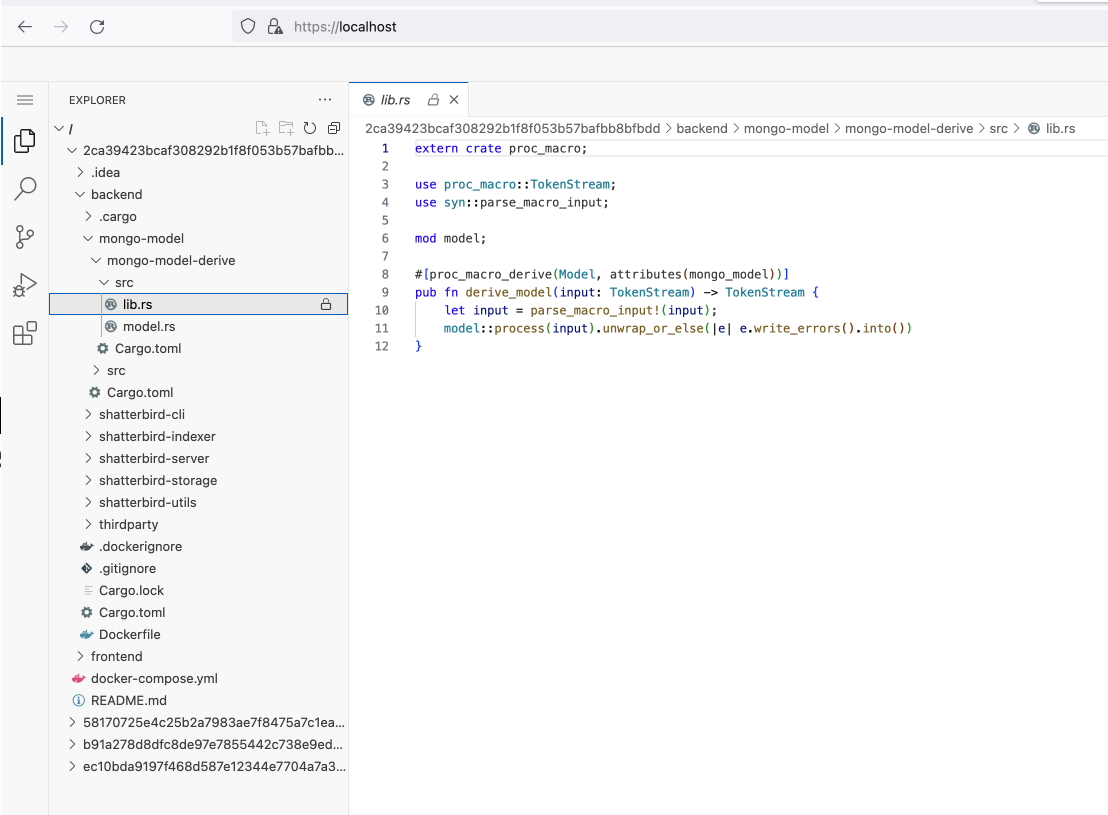
\includegraphics[width=\textwidth,height=0.5\textheight,keepaspectratio]{figures/intro.png}
    \caption{Скриншот пользовательского интерфейса, доступного по протоколу https}
\end{figure}

\section{Процесс индексирования}

Индексация репозитория разделяется на два этапа: загрузка объектов Git и загрузка данных результата индексации в формате LSIF. Оба этих этапа можно осуществлять с помощью программы \texttt{shatterbird-indexer}.

Во-первых, рассмотрим процесс загрузки объектов Git. Для загрузки объектов репозитория необходимо указать строку подключения к базе данных и путь к корню репозитория. Сам же процесс загрузки можно описать следующим алгоритмом:

\begin{enumerate}
    \item Найти текущий коммит в репозитории и проверить его наличие в базе данных. Если уже был загружен, то алгоритм можно завершить.
    \item Если у него есть родительские коммиты, то выполнить этот алгоритм рекурсивно, используя в качестве текущего коммита по очереди каждый из родительский. Можно не выполнять рекурсивно, если глубина загрузки истории уже больше, чем максимально указанная пользователем.
    \item Найти корневую директорию этого коммита и убедимся, что она не загружена в базу данных. Назовём её текущей.
    \item \label{git-upload-algo-dir-1} Для всех файлов в текущей директории проверить их наличие в базе данных. Если файл отсутствует, то загрузить его и все содержащиеся в нём строки. В этот момент возможно загрузить из базы данных предыдущие версии файла (из родительских коммитов) и переиспользовать ранее существовашие строки, чтобы сохранить построенные для них индексы.
    \item \label{git-upload-algo-dir-2} Для всех директорий в текущей директории также проверить наличие в базе данных. Если директория отсутствует, то выполнить рекурсивно пункты \ref{git-upload-algo-dir-1}-\ref{git-upload-algo-dir-2}, используя по очереди каждую ещё не загруженную директорию в качестве текущей.
    \item После того как корневая директория и все её потомки были загружены в базу данных, необходимо также загрузить объект коммита, включая в него ссылки на его родителей и ссылку на корневую директорию. Если какой-либо из родителей не был загружен в базу данных, то их нужно пропустить.
\end{enumerate}

В итоге в базе данных дублируются объекты Git-репозитория с использованием моделей, описанных в приложении \fullref{addendum:models}. А именно, используются объекты \texttt{Commit} для описания объектов коммитов и объекты \texttt{Node} для описания файлов и директорий.

Во-вторых, рассмотрим алгоритм загрузки графа LSIF в базу данных. Для этого на вход программе подается граф в виде списка JSON-строк: можно загрузить из файла, а можно прочитать из стандартного входа. Также необходимо в параметрах командной строки указать строку подключения к базе данных.

\begin{enumerate}
    \item Сначала необходимо загрузить граф из файла в память. При этом запоминаются все вершины графа, а для каждого также составляется список ребёр \textbf{исходящих} из него. Сразу дополнительно собирается список ссылок на те вершины, которые отражают документы (файлы).
    \item Затем для каждой вершины-документа из графа в Git-репозитории ищется соответствующей ей объект файла. Это позволяет сопоставить каждую вершины-документа с ранее загруженным в базу данных файловым объектом.
    \item Для каждой вершины типа «Range» ищется соответствующий ему файл, а в нём — нужная строка. Это необходимо, потому что файлы хранятся как массив строк, к которым и привязывается граф. Затем в базе данных подготавливается объект Range, содержащий идентификатор строки, начало и конец отрезка в ней, а также полный путь к этому файлу, начиная от корневой директории и заканчивая найденным файлом. Путь хранится как массив идентификаторов соответствующих объектов Node в базе данных.
    \item Наконец, запускается рекурсивный обход графа в глубину, начиная с каждой из вершин-документов. При этом все посещаемые вершины получают уникальный ObjectID (совместимый с MongoDB) и конвертируются в структуру, совместимую с хранимой в базу данных моделью данных. Аналогично обрабатываются ребра графа, но только после посещения всех вершин, которые связывает каждое отдельное ребро.
    \item Затем все эти объекты загружаются в базу данных.
\end{enumerate}

Для реализации этого алгоритма на языке Rust используется паттерн «Arena», который заключается в аллокации всех элементов графа (вершин и ребер) в одной структуре с единым временем жизни. Это позволяет легко гарантировать, что ребра, содержащие ссылки на вершины, будут все уничтожены одновременно с вершинами графа. Таким образом содержащиеся в ребрах ссылки никогда не будут висячими. Хотя такой подход и не позволяет освобождать память у отдельных объектов, но в данном случае этого и не требуется.

Благодаря использования итераторов и использования потокобезопасных коллекций, многие этапы алгоритма выполняются параллельно и используют все доступные потоки процессора.

\section{Инструмент для отладки}

Также во время работы над проектом был разработан вспомогательный инструмент для облегчения отладки и разработки системы. Он позволяет визуализировать граф, находящиеся в базе данных.

При запуске инструмента указывается идентификатор вершины графа, окрестности которого необходимо визуализировать. Затем, используя данные из базы данных, производится обход графа от этой вершины. Осуществляется поиск всех входящих рёбер и всех исходящих рёбер. Затем рекурсивно посещаются вершины по другую сторону кадждого ребра. Причем вершины типов Document и Moniker пропускаются, поскольку они связаны с большим количеством других вершин и значительно усложняют восприятие графа.

В процессе этого обхода каждое ребро и вершины записываются в формате dot для дальнейшей визуализации, причем начальная вершина дополнительно выделяется цветом, а все рёбра и вершины получают подписи с их типом. Дополнительно для вершин типа «Range» (то есть, указывающих на подстроки в файлах) добавляется подпись, содержащая эту подстроку и номер строки, в которой она содержится. Имя файла для таких вершин доступно при наведении курсора на вершину (при просмотре получившегося SVG файла).  После того как обход графа был завершен, полученный файл в формате dot преобразуется в SVG с использованием установленной на компьютере утилиты \texttt{neato}.

Важной особенностью утилиты является возможность выводить получившееся изображение прямо в терминал, с использованием специальных расширений (поддерживаются эмуляторы терминала iTerm2 и Kitty). При необходимости вывода на экран полученное SVG-изображение сперва преобразуется в растровое в формате PNG c помощью библиотеки resvg.

Примером работы программы является рис. \ref{fig:lsif-graph}.

\section{Описание контейнеров для запуска проекта}

Для облегчения запуска системы, используется система контейнеризации Docker и утилита docker-compose. Это позволяет обеспечить воспроизводимую сборку системы, а также позволяет описать все параметры конфигурации  и запуска в файлах, которые затем будут версионироваться и распространяться вместе со всем остальным кодом проекта.

Сборка серверной части описывается в Dockerfile, состоящим из этапа сборки и трех этапов, копирующих скомпилированные файлы для создания отдельных образов под разные программы: cli, indexer и server. Такой подход позволяет одновременно выполнить достаточно трудоемкое скачивание зависимостей и компиляцию только однажды при сборке первого этапа и при этом не включать исходные коды и промежуточные артефакты сборки вместе с конечными образами контейнеров — те содержат только единственный бинарный файл с соответствующим образу программой.

Сборка клиентской части также является многоэтапной: на первом этапе скачиваются все зависимости и собираются файлы сайта, а второй этап копирует получившийся результат в финальный образ, а также включает в него веб-сервер Caddy и его конфигурацию.

Наконец, все эти образы координируются с помощью файла docker-compose.yml, который позволяет при сборке указывать тег для каждого собранного образа, а также описывает конфигурацию запуска всей системы. Система состоит из трёх контейнеров: бекенд, база данных и фронтенд. При этом доступ к базе данных часто нужен из вспомогательных контейнеров при индексации, а фронтенд взаимодействует только с бекендом. Поэтому в рамках docker-compose описываются две сети: front и back. В первую сеть включен только фронтенд и бекенд, а во вторую — только бекенд и база данных. При этом предполагается, что в сети back также будут запускаться короткоживущие контейнеры при загрузке новых индексов.

Также docker-compose.yml описывает запуск контейнера с базой данных MongoDB. Для обеспечения персистентности данных, объявляется и используются специальный том «mongo-data», в котором хранятся данные. Аналогично при помощи тома обеспечивается персистентность для обратного прокси — тот сохраняет на диск информацию о полученных TLS-сертифкатов и эти данные должны сохраняться между перезапусками контейнера.

Для того, чтобы дать вспомогательным образам indexer и cli имена, они также упоминаются в файле docker-compose.yml, но отмечены для использования только в профиле сборки. Таким образом при запуске системы с помощью обычного профиля они не будут каким-либо образом использоваться, но участвуют в сборке и получают в её процессе имена.

Наконец, чтобы облегчить пользователю развертывание системы, файл конфигурации обратного прокси Caddy устроен так, что позволяет указать домен с помощью переменной окружения. Таким образом, при развертывании системы достаточно только указать в docker-compose.yml используемый домен (например, «\texttt{example.org}»), чтобы веб-сервер автоматически обрабатывал запросы только для этого домена и получил для него TLS-сертификат.

\section{Документирование исходного кода и юнит-тесты}

Для серверной части используются встроенные в стандартную поставку языка инструменты для документирования и тестирования. Это позволяет с использованием команды «\texttt{cargo doc}» автоматически сгенерировать документацию ко всем типам, а с помощью команды «\texttt{cargo test}» запустить все юнит-тесты. При этом код юнит-тестов не включен в релизную сборку и не увеличивает размер бинарного файла, не ухудшает быстродействие программы и не увеличивает время компиляции. Эта особенность тестов и простота их запуска также позволяет во время запуска тестов автоматически обновлять сгенерированные описания моделей данных на языке Typescript для их дальнейшего использования в коде клиентской части.

Код клиентской части, написанный на языке Typescript, не применяет никаких инструментов для документации и юнит-тестирования, поскольку объем кода достаточно небольшой, а юнит-тестирование расширения для Visual Studio Code достаточно трудоемко.

\section{Выводы по главе}

В этой главе были подробны описаны детали реализации системы: общая архитектура и структура проекта, приведено описание всех лежащих в её основе отдельных программ. Приводится подробное описание алгоритма индексирования и устройство работы пользовательского интерфейса, а также описаны особенности эффективного данных. Наконец, описывается взаимодействие отдельных компонентов друг с другом и приводится использование Docker для сборки и запуска проекта.

\clearpage

	\addchap{Заключение}
\label{chap:final}

Благодаря данной выпускной квалификационной работе, была разработана открытая и бесплатная система, облегчающая работу разработчиков программного обеспечения. Такая система позволяет им более продуктивно изучать исходный код незнакомых проектов и быстрее находить в нём ответы на свои вопросы. Причем система является расширяемой и может поддерживать многие языки программирования, а также проста в развертывании и использовании. 
\medskip

В процессе работы над проектом были решены следующие задачи:

\begin{enumerate}
    \item Получение исходных текстов из Git-репозитория, эффективно используя особенности этой системы контроля версий;
    \item Получение семантической информации с использованием результатов работы любого корректного индексатора, поддерживающего формат LSIF;
    \item Хранение полученных данных в базе данных MongoDB, в том числе с использованием индексов для ускорения читающих запросов;
    \item Реализован веб-интерфейс на базе Visual Studio Code, использующий эти данные для отображения пользователю исходные текстов и предоставляющий расширенный функционал навигации;
    \item Простота развертывания достигается благодаря использованию файлов Dockerfile и docker-compose, описывающих процесс сборки и процедуру запуска системы;
\end{enumerate}

\medskip

В том числе существует несколько направлений дальнейшего развития этой работы:
\begin{enumerate}
    \item Разработка инструментария для автоматического запуска индексирования репозитория. На данный момент предлагается интеграция с используемыми в проекте системами CI/CD.
    \item Разработка модели разграничения доступов к отдельным файлам или директориям репозиториев.
    \item Улучшения интеграции интерфейса с системой контроля версий Git: поддержка функций «annotate» (кто последний менял ту или иную строку), просмотр списка коммитов и веток.
    \item Поддержка быстрого текстового поиска по репозиторию с использованием regexp.
\end{enumerate}

\clearpage
	% \phantomsection
% \addcontentsline{toc}{chapter}{}

\oldaddsec[\\\hspace*{-1cm}Список использованной литературы]{\hfill{Список использованной литературы}\hfill\mbox{}}

\printbibliography[heading=none,type=book]

\bigskip

\printbibliography[heading=none,nottype=book,nottype=online]

\bigskip

\printbibliography[heading=none,type=online]

\clearpage
 % Ручками редактировать не надо, лучше юзать bibtex (см. bibliography.bib)

    % Ниже следуют приложения
    \setcounter{chaps}{\value{chapter}}
    \appendix
    \renewcommand{\chapterformat}{Приложение \Asbuk{chapter}:\enskip}
    
	\addendum{Модели объектов}
\label{addendum:models}

Это приложение содержит описание моделей, используемых в проекте. Все модели описаны с помощью языка Typescript. Тип \texttt{Id<T>} обозначает идентифкатор объекта типа \texttt{T}.

\section{Модели для содержимого Git-репозитория}

Эти модели используются для хранения файлов и директорий Git-репозитория в базе данных:

\begin{itemize}
    \item Коллекция \texttt{commits}:
        \begin{minted}[gobble=8]{TypeScript}
        /**
         * Объект коммита, импортированного из Git-репозитория
         */
        export type Commit = { 
            /**
             * Идентификатор объекта в базе данных
             */
            _id: Id<Commit>, 
            
            /**
             * Хранит хэш, который используется для идентификации соответствующего объекта в Git
             */
            oid: string, 
            
            /**
             * Идентификатор корневой директории репозитория
             */
            root: Id<Node>, 
            
            /**
             * Список коммитов-родителей, если они также загружены в хранилище
             */
            parents: Array<Id<Commit>>,
        }
        \end{minted}

    \item Коллекция \texttt{nodes}:
        \begin{minted}[gobble=8]{TypeScript}
        /**
         * Объект в файловом дереве
         */
        export type Node = {
            /**
             * Идентификатор объекта в базе данных
             */
            _id: Id<Node>,
            
            /**
             * Хранит хэш, который используется для идентификации соответствующего объекта в Git
             */
            oid: string,
            
            /**
             * Содержимое объекта, в зависимости от его типа
             */
            content: {
                "Symlink": {
                    /**
                     * Путь, на который ссылается эта ссылка
                     */
                    target: string,
                }
            } | {
                "Directory": {
                    /**
                     * Объекты. входящие в эту директорию и их имена
                     */
                    children: { [key: string]: Id<Node> },
                }
            } | {
                "Text": {
                    /**
                     * Суммарный размер файла
                     */
                    size: bigint,
                    
                    /**
                     * Список строк, входящих в этот файл
                     */
                    lines: Array<Id<Line>>,
                }
            } | {
                "Blob": {
                    /**
                     * Суммарный размер файла
                     */
                    size: bigint,
                    
                    /**
                     * Идентификатор объекта, содержащего этот файл
                     */
                    content: Id<BlobFile>,
                }
            },
        };
        \end{minted}
        
    \item Коллекция \texttt{blobs}:
        \begin{minted}[gobble=8]{TypeScript}
        /**
         * Содержимое файла, который не удалось разделить на отдельные строки
         */
        export type BlobFile = {
            /**
             * Идентификатор объекта в базе данных
             */
            _id: Id<BlobFile>,
            
            /**
             * Содержимое файла (байты)
             */
            data: Array<number>,
        };
        \end{minted}
    
    \item Коллекция \texttt{lines}:
        \begin{minted}[gobble=8]{TypeScript}
        /**
         * Содержимое отдельной строки текстового файла
         */
        export type Line = {
            /**
             * Идентификатор объекта в базе данных
             */
            _id: Id<Line>,
            
            /**
             * Строка
             */
            text: string,
        };
        \end{minted}
\end{itemize}

\section{Модели для результатов индексирования}

Эти модели используются для хранения результатов работы LSIF в базе данных:

\begin{itemize}
    \item Коллекция «lines»:
        \begin{minted}[gobble=8]{TypeScript}
        /**
         * Описание подстроки в файле
         */
        export type Range = {
            /**
             * Идентификатор объекта в базе данных
             */
            _id: Id<Range>,
            
            /**
             * Идентификатор строки, в которой находится подстрока
             */
            line_id: Id<Line>,
            
            /**
             * Полный путь к этому файлу
             */
            path: Array<Id<Line>>,
            
            /**
             * Индекс первого символа подстроки
             */
            start: number,
            
            /**
             * Индекс конца подстроки
             */
            end: number,
        };
        \end{minted}
    
    \item Коллекция «edges»:
        \begin{minted}[gobble=8]{TypeScript}
        /**
         * Ребро графа, связывающее те или иные вершины
         */
        export type Edge = {
            /**
             * Идентификатор объекта в базе данных
             */
            _id: Id<Edge>,
            
            /**
             * Информация об ребре, предоставленная LSIF
             */
            data: {
                /**
                 * Вид ребра
                 */
                edge: "Contains"
                    | "Moniker"
                    | "NextMoniker"
                    | "Next"
                    | "PackageInformation"
                    | "Item"
                    | "Definition"
                    | "Declaration"
                    | "Hover"
                    | "References"
                    | "Implementation"
                    | "TypeDefinition"
                    | "FoldingRange"
                    | "DocumentLink"
                    | "DocumentSymbol"
                    | "Diagnostic",
                    
                /**
                 * Входящая вершина, если один
                 */
                in_v?: Id<Vertex>,
                
                /**
                 * Входящие вершины, если несколько
                 */
                in_vs?: Array<Id<Vertex>>,
                
                /**
                 * Исходящая вершина
                 */
                out_v: Id<Vertex>,
            },
        };
        \end{minted}
        
    \item Коллекция «vertices»:
        \begin{minted}[gobble=8]{TypeScript}
        /**
         * Вершина графа
         */
        export type Vertex = {
            /**
             * Идентификатор объекта в базе данных
             */
            _id: Id<Vertex>,
            
            /**
             * Информация об вершине, предоставленная LSIF
             */
            data: {
                /**
                 * Вид вершины
                 */
                vertex: "MetaData"
                      | "Project"
                      | "Document"
                      | "Range"
                      | "ResultSet"
                      | "Moniker"
                      | "PackageInformation"
                      | "DefinitionResult"
                      | "DeclarationResult"
                      | "TypeDefinitionResult"
                      | "ReferenceResult"
                      | "ImplementationResult"
                      | "FoldingRangeResult"
                      | "HoverResult"
                      | "DocumentSymbolResult"
                      | "DocumentLinkResult"
                      | "DiagnosticResult",
                
                // Также содержит дополнительные поля, зависящие от конкретного вида вершины.
            },
        };
        \end{minted}
\end{itemize}

\section{Объект FullNode}
\label{models:fullnode}

Этот объект не хранится в базе данных, но используется при взаимодействии с клиентской частью.

\begin{minted}{TypeScript}
/**
 * Хранит полную информацию об узле файлового дерева
 */
export type FullNode = {
    /**
     * Идентифкатор этого узла в базе данных
     */
    _id: Id<Node>,

    /**
     * Тип узла
     */
    kind: "Symlink" | "Directory" | "Text" | "Blob",

    content: {
        "Symlink": {
            /**
             * Ссылка на целевой файл
             */
            target: string,
        }
    } | {
        "Directory": {
            /**
             * Дочерние узлы этой директории вместе с их именами
             */
            children: {
                [key: string]: {
                    /**
                     * Идентифкатор этого узла в базе данных
                     */
                    _id: Id<Node>,
                    
                    /**
                     * Тип узла
                     */
                    kind: "Symlink" | "Directory" | "Text" | "Blob",
                }
            },
        }
    } | {
        "Text": {
            /**
             * Размер файла в байтах
             */
            size: bigint,
            /**
             * Строки файла
             */
            lines: Array<{
                /**
                 * Идентификатор объекта в базе данных
                 */
                _id: Id<Line>,
                
                /**
                 * Текст строки
                 */
                text: string,
            }>,
        }
    } | {
        "Blob": {
            /**
             * Размер файла в байтах
             */
            size: bigint,
            
            /**
             * Идентификатор этого файла в базе данных
             */
            content: Id<BlobFile>,
        }
    },
};
\end{minted}


\clearpage
	\addendum{Содержимое репозитория}
\label{addendum:repo}

\begin{verbatim}
.
├── README.md
├── backend
│   ├── Cargo.lock
│   ├── Cargo.toml
│   ├── Dockerfile
│   ├── mongo-model
│   │   ├── Cargo.toml
│   │   ├── mongo-model-derive
│   │   │   ├── Cargo.toml
│   │   │   └── src
│   │   │       ├── lib.rs
│   │   │       └── model.rs
│   │   └── src
│   │       ├── id.rs
│   │       └── lib.rs
│   ├── shatterbird-cli
│   │   ├── Cargo.toml
│   │   └── src
│   │       ├── graph.rs
│   │       └── main.rs
│   ├── shatterbird-indexer
│   │   ├── Cargo.toml
│   │   └── src
│   │       ├── exclusive.rs
│   │       ├── git
│   │       │   └── mod.rs
│   │       ├── lsif
│   │       │   ├── converter.rs
│   │       │   ├── graph.rs
│   │       │   ├── lsif_ext.rs
│   │       │   └── mod.rs
│   │       └── main.rs
│   ├── shatterbird-server
│   │   ├── Cargo.toml
│   │   └── src
│   │       ├── filesystem
│   │       │   ├── mod.rs
│   │       │   └── model.rs
│   │       ├── language_server
│   │       │   ├── error.rs
│   │       │   ├── methods.rs
│   │       │   └── mod.rs
│   │       ├── main.rs
│   │       ├── settings.rs
│   │       ├── state.rs
│   │       └── utils.rs
│   ├── shatterbird-storage
│   │   ├── Cargo.toml
│   │   └── src
│   │       ├── lib.rs
│   │       ├── model
│   │       │   ├── files.rs
│   │       │   ├── lang.rs
│   │       │   └── mod.rs
│   │       ├── serializers
│   │       │   ├── gix_hash.rs
│   │       │   └── mod.rs
│   │       ├── ts.rs
│   │       └── util
│   │           ├── graph.rs
│   │           └── mod.rs
│   └── shatterbird-utils
│       ├── Cargo.toml
│       └── src
│           ├── cli.rs
│           └── lib.rs
├── docker-compose.yml
└── frontend
    ├── Caddyfile
    ├── Dockerfile
    ├── README.md
    ├── dev.js
    ├── package.json
    ├── pnpm-lock.yaml
    ├── public
    │   ├── index.html
    │   ├── product.json
    │   └── shatterbird
    │       └── package.nls.json
    ├── src
    │   ├── extension.ts
    │   ├── filesystem
    │   │   ├── fsClient.ts
    │   │   ├── fsProvider.ts
    │   │   ├── fsProviderBase.ts
    │   │   ├── fsRoot.ts
    │   │   ├── node.ts
    │   │   ├── repoRoot.ts
    │   │   └── types.ts
    │   ├── language
    │   │   └── languageClient.ts
    │   ├── manifest.json
    │   └── server-types
    │       ├── BlobFile.ts
    │       ├── Commit.ts
    │       ├── ContentKind.ts
    │       ├── Edge.ts
    │       ├── EitherNode.ts
    │       ├── ExpandedFileContent.ts
    │       ├── FileContent.ts
    │       ├── FullNode.ts
    │       ├── Id.ts
    │       ├── Line.ts
    │       ├── Node.ts
    │       ├── NodeInfo.ts
    │       ├── Range.ts
    │       └── Vertex.ts
    ├── tsconfig.json
    └── vite.config.ts

30 directories, 80 files
\end{verbatim}
\end{document}